\chapter{Vyhledávání}
\label{kap:vyhledavani}

Možnost vyhledávat v~nahrávkách byl pro mne jeden z~hlavních cílů od začátku
projektu. Se~získáním přepisů náhrávek, byť kolísavé kvality, bylo možné
vyhledávání realizovat.
Fulltextové vyhledávání jsem implementoval nástroje Elastic.

Elastic je svobodný vyhledávač napsaný v~Javě, který umožňuje fulltextové
vyhledávání v~dokumentech. Dokumenty se rozumí datové struktury, které se
vyhledávači poskytnou ve formátu JSON. Elastic má mnoho funkcionalit,
z~nichž pro mne je klíčové rozhraní na základě HTTP naplňující konvence REST,
automatický stemming, zvýrazňování nalezených pasáží a možnost vyhledávat
v~libovolných položkách dokumentu.

Aby bylo možné každý nalezený výsledek proměnit v~odkaz na příslušnou pasáž
v~nahrávce, zvolil jsem za jednotlivé dokumenty nikoliv celé nahrávky, nýbrž
věty.

Ke každému dokumentu se ukládá
\begin{itemize}
\item{textová reprezentace,}
\item{posloupnost hlásek,}
\item{stupeň
manuálního přepisu, tedy zda je přepis pořízen zcela automaticky, zcela manuálně
nebo kombinací obého}
\item{a také vektor confidence measure jednotlivých automaticky přepsaných slov.}
\end{itemize}

Pro skloňování je použito pravidlového stemmingu, který je dodáván s~distribucí
Elastic a pro češtinu, obzvlášť tam, kde se vyskytuje mnoho
nestandardních a archaických slov, funguje báječně.

Momentálně je vyhledávač nainstalován na témž serveru jako API a je dostupný
z~webové aplikace. Důležitým bodem budoucí práce je automatizace indexování
manuálních oprav, jak přicházejí. Dále pak zakomponování automatického přepisu
pořízeného bez použití jazykového modelu, jak se diskutuje
v~podsekci~\ref{ssec:data:topicsearch}.

\section{Kvantitativní vyhodnocení}

Do jaké míry lze současný přepis použít k~vyhledávání v~korpusu? To jsem se
pokusil odhadnout jednak na testovací sadě a jednak namátkou.

Na testovací sadě jsem vyhodnocení provedl tak, že jsem vzal všechna podstatná
jména vyskytující se v~ní a vyhledal je v~ručním i v~automatickém přepisu.
Za úspěch jsem považoval, byla-li daná {\em věta} mezi výsledky v~obou
případech.

Podstatná jména jsem převedl do regulárních výrazů reflektujících skloňování.
Celkem byly 344. Vět bylo celkem 376 s~5511 tokeny. Každé slovo se samozřejmě
mohlo vyskytnout v~mnoha větách. Zásahů mezi větami v~automatickém přepisu bylo
840, mezi větami v~ručním 880 a úspěšných zásahů bylo 813, což znamená \textbf{precision
96,79\% a recall 92,39\%}.

\subsection{Identifikace témat}
\label{ssec:data:topicsearch}

Provedl jsem dva ,,baselinové`` pokusy o automatickou identifikaci témat
v~mluveném korpusu, které jsou popsány v~článku Krůza (2019)\cite{kruza2019spoken}

První z~nich využívá toho, že pojmenované entity a některé další výrazy se běžně
nevyskytují v~řeči, pokud se nemluví právě o nich. Vybral jsem namátkou klíčová
slova
\begin{enumerate}
\item{Lazar,}
\item{Mithra, mithraismus,}
\item{Satan,}
\item{svatá Terezie,}
\item{pohádka.}
\end{enumerate}

Pohádku jsem vybral jakožto opakující se téma, které není vázané na pojmenovanou
entitu, ačkoliv by bývalo šlo použít jméno Honza, které se u Makoně vyskytuje
obvykle právě ve spojitosti s~pohádkou.

V~přepisu %, kde je přibližně 100 hodin přepsáno ručně a zbytek více než tisíce hodin automaticky,
získaném pomocí neuronových sítí trénovaných na manuálním přepisu Makoňova korpusu jsem vyhledal kmeny
výše zmíněných slov. Výsledek hledání shrnuje tabulka~\ref{tab:topicsearch}.
U výsledků jsem manuálně zkontroloval, je-li tématem skutečně hledaný výraz.
Pokud bylo výsledků hledání více než 20, zkontroloval jsem toto u náhodných
dvaceti výsledků.

\begin{table}[htpb]
\begin{center}
\begin{tabular}{|l|l|r|r|r|r|}
\hline
téma &
dotaz &
\makecell{výsledků\\ v~automat.\\ přepisu} &
\makecell{očekávaný\\ počet výsl.\\ v~aut. přep.} &
\makecell{výsledků\\ v~manuálním\\ přepisu} &
precision \\
\hline
Lazar & \texttt{lazar.*} & 113 & 157 & 14 & 11/20   \\
Mithra & \texttt{mith?ra.*} & 0 & 0 & 0 & n/a   \\
Satan & \texttt{satan.*} & 1659 & 1741 & 155 & 14/20   \\
Sv. Tereza & \texttt{terez.*} & 1906 & 1752 & 156 & 14/20   \\
pohádka & \texttt{pohádk.*} & 911 & 640 & 57 & 16/20   \\
\hline
\multicolumn{5}{|l|}{celková precision} & 68,75\%\\
\hline
\end{tabular}
\caption{Výsledky textového vyhledávání v~přepisu v~prosinci 2020. Precision počítána pouze
z~automatických přepisů.}\label{tab:topicsearch}
\end{center}
\end{table}

% *: h: 718097, a: 8069250
% lazar: h: 14, a: 127  - 3 17 + PLZEŇ!!! ; jeden dobrý přepis, ne téma
% mithra: h: 0, a: 0
% satan: h: 155, a: 1814    - 3 17 +    Plzeň!
% tereza: h: 156, a: 2062   - 1 19 +    Tereza ~ které za
% pohádka: h: 58, a: 1014   - 0 20 +    Plzeň!

Precision 69\% poukazuje na fakt, že
kvalita přepisu umožňuje v~korpusu rozumně vyhledávat.
Navíc pouze polovina chyb byla způsobena špatným přepisem. Zbylou polovinu
tvořily případy, kdy se dané slovo skutečně v~mluvě vyskytlo, ale jen jako letmá
zmínka.

Celkem 8,9\% slov v~korpusu bylo v~době tohoto experimentu manuálně přepsáno. Sloupec ,,očekávaný počet
výsledků v~automatickém přepisu`` obsahuje interpolaci toho, kolik výsledků by
mělo být obsaženo, pokud by frekvence byla stejná jako v~manuálním přepisu.
Je vidět, že očekávaný a nalezený počet výskytů se příliš neliší, což napovídá,
že recall je není vyloženě žalostný.

Jeden falešný
výsledek hesla {\em ,,lazar``} spočíval v~použití tohoto slova pro označení
nemocného člověka, tedy v~přeneseném významu. Zde se tedy odrazila omezenost
této metody pro hledání tématu, nikoliv nedokonalost přepisu. Při zkoumání
výsledků vyhledávání hesla {\em ,,tereza``} v~podobě regulárního výrazu
\texttt{terez.*} jsem dospěl ke kurióznímu zjištění: Když nalezený výskyt byl
formou slova {\em ,,Terezie``}, výsledek byl vždy správný, nenarazil jsem na žádnou
výjimku. Ovšem byl-li výsledek {\em ,,Tereza`` }, šlo ve více než polovině případů o
chybně přepsaná slova {\em ,,které za``}. Forma {\em ,,Terezie``} je v~přepisu
pětadvacetkrát častější, takže na výsledku tohoto experimentu se tato chyba
odrazila jen nepatrně.

Díky tomu, že mithraismus se vyskutuje v~ručních indexech k~nahrávkám, lze se
přesvědčit, v~čem tkví nulový výskyt tohoto hesla v~přepisech. Automatický
přepis zde skutečně selhává, vole slova jako {\em ,,mistrů``} místo {\em
,,Mithrův``} nebo {\em ,,my trasu``} místo {\em ,,mithraismus``}. Pokusil jsem
se několik frází obsahujících nějaké slovo odvozené od jména ,,Mithra``
rozpoznat bez použití jazykového modelu. Např. pro frázi {\em ,,se v~jejich
kultu mithraistickém znázorňovala``} se bez jazykového modelu dojde k~predikci
{\em ,,te jejích kultu mitra jistickém znázorňovala``}.

Zdá se proto, že by bylo užitečné mít k~dispozici pro vyhledávání i přepis
získaný bez použití jazykového modelu. Toto je předmětem budoucí práce.

\subsection{Korelace témat mezi nahrávkami a knihami}

Pro vyhledávání se dá využít i psaných Makoňových děl. Věc se zakládá na
domněnce, že v~době, kdy Makoň o určitém tématu psal knihu, o něm bude
pravděpodobně také mluvit na přednáškách. Pro ověření domněnky jsem se zaměřil
na téma svaté Terezie z~Avily. V roce 1988 Makoň překládal její dílo {\em Hrad nitra
(El castillo interior)}. Vzhledem k~tomu, že u většiny nahrávek známe rok jejich
pořízení, lze zjistit distribuci výskytů vyhledávání podle roku. Pro dotaz na
svatou Terezii tuto distribuci ukazuje obrázek~\ref{fig:teresa-year}.

\begin{figure}[htpb]
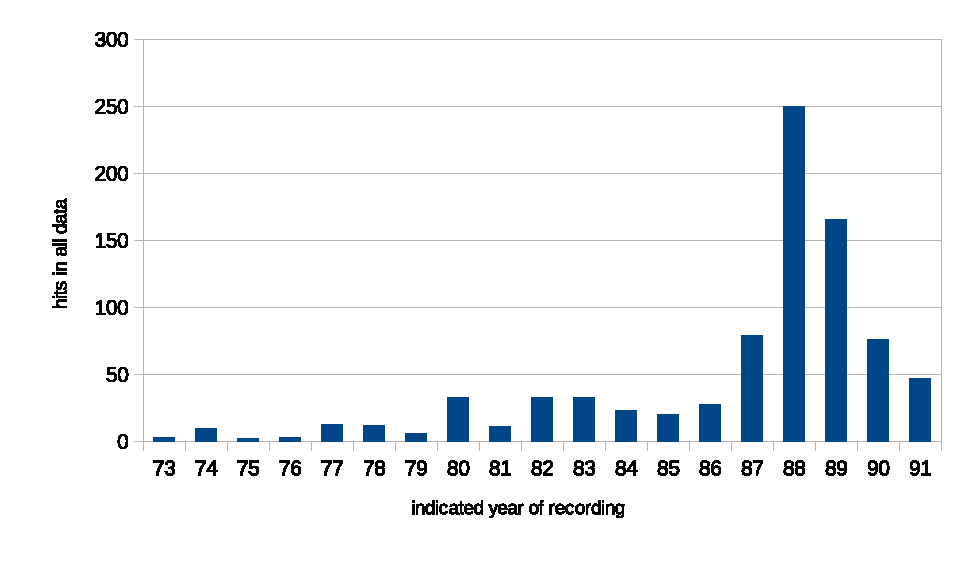
\includegraphics[scale=0.9]{rc/teresa-by-year.eps}
\caption{Počet výsledků vyhledání dotazu \texttt{terez.*} v~přepisech podle
udaného roku nahrávky.}
\label{fig:teresa-year}
\end{figure}

Elevace kolem roku 1988 v~grafu domněnku korelace mezi tématem právě psané knihy
a tématem přednášek podporuje.



\section{Případová studie}

Vyhledávání v~přepisech mluveného korpusu našlo využití v~kompilaci referátů o
určitých tématech, kterým se Karel Makoň věnuje. V průběhu let 2018 až 2020
vznikly alespoň čtyři takové, a to na témata
\begin{itemize}
\item{karma,}
\item{převtělování,}
\item{Otčenáš,}
\item{relativní dobro a zlo.}
\end{itemize}
Každé téma bylo zpracováno do formy souboru krátkých úseků nahrávek, které se
prezentovaly sekvenčním přehráním s~podporou přepisů jako zrakového vodítka.

Autor referátu o tématu relativního dobra a zla dohledal poznámkový aparát
k~tvorbě a rekonstruoval svůj postup, který zde popíšu jako příklad použití
přepisů, z~něhož lze usoudit na efektivitu práce.

Téma relativního dobra a zla bylo předem zamyšleno a bylo vybráno pro autorův
zájem a nikoliv s~ohledem na to, jak snadné bude pro vyhledání. Dopředu byl dán
časový rámec výsledku na cca. dvě hodiny zvukového záznamu.

Autorova metodika byla následovná: vyhledal frázi ,,relativní dobro a zlo`` a
výsledky procházel ve výchozím relevančním řazení nástroje Elastic. Prošel
prvních sto z~celkových 7379 výsledků. U každého posoudil, zda se jedná o
pasáž, skutečně o tématu pojednávající, nebo jen o letmou zmínku či vůbec
falešný zásah, popřípadě o duplicitní výskyt.

Výběr vzorků probíhal ve dvou průchodech. V~prvním autor vybíral relevantní a
relativně obsáhlejší zásahy, čímž se tvořila užší množina kandidátských úseků.
V~druhém průchodu pak vybíral z~této užší množiny s~ohledem na ročník zdrojové
nahrávky, aby byl v~kompilátu zastoupen průřez vývoje Makoňova myšlení,
výjimečně podle návaznosti či pro závěrečnou část shrnující charakter výpovědi.

Po prvním průchodu se do užšího výběru dostalo 25 nalezených úseků, tedy
čtvrtina procházené množiny, a všechny byly z~prvních 53 zásahů. V~první stovce
výsledků vyhledávání autor identifikoval 16 duplicit.
